\documentclass[11pt]{IEEEtran}

\usepackage{cite}				% Used to cite references and figures
\usepackage{titling}			% Used to move title up when not in IEEEtran
\usepackage{subcaption}			% Used to add captions to subfigures
\usepackage{graphicx}			% Used to import pdf images
\usepackage{float}				% Used to keep images where they are defined using [H] tag
\usepackage{amsmath}			% Used for equation reference
\usepackage{amsfonts}			% Used for equation symbols
\usepackage[export]{adjustbox}	% Used to left align selected figures
\usepackage{siunitx} 			% Used to align decimals in table and for degree symbl \ang{}
\usepackage{hyperref}
\usepackage{bookmark}
\usepackage{algorithm,algpseudocode}			% Used to create an algorithm block
\usepackage{pgfgantt}
\usepackage{tabularx}			% Allows for double-column spanning table
\usepackage{dblfloatfix}		% Allows figure* to be at bottom of page


% Change section autoref label from 'section' (default) to 'Section'
\renewcommand*{\thesection}{\Roman{section}}


\hypersetup{
	colorlinks = true,
	linkcolor = blue,
	filecolor = magenta,
	urlcolor = black,
	citecolor = blue,
	pdftitle = {Autonomous Tread Identification System},
	pdfpagemode = UseOutlines,
}

\begin{document}

	\title{ \vspace{-0.0575in} Autonomous Tread Identification System }

	\author{	Senior Design I Student Proposal \\
				University of North Texas Department of Electrical Engineering \\
				EENG 4910.001 \\ \\
				Nicholas Chiapputo, Brandon Jones, Tim McCoig, Samuel Simmons \\
				Faculty Advisor: Colleen Bailey, PhD
	}

	\maketitle

	% \begin{abstract}
	% \end{abstract}

	\section{Problem Definition}
		Tire-related issues, including blowouts, tread separation, and worn tread, are some of the most common causes of vehicle accidents. In 2015, more than 35,000 people died from motor vehicle accidents in the United States alone. For every person killed in a motor vehicle accident, 8 people were hospitalized and 99 people were treated and released from emergency departments \cite{cdcKeyStats}. The NHTSA has reported that on tire-related crash vehicles, 26.2\% of tires had a tread-depth of the legal minimum of 2/32'' or less \cite[pp.~8-9]{nhtsaCrashStats}. We propose an autonomous tire tread sensor to alert vehicle operators to uneven or dangerous tread on their tires.

		\subsection{Background}
			A tire is made up mostly of rubber and has built-in innovative securities to allow the rubber to have traction on road surfaces. The main addition to the rubber on a tire is called tread. The tread of the tire is what contacts the driving surface and has been engineered to grab or grip the surface it impacts and travels on. It is developed by creating unique designs on the surface on the circumference of the tire. The tread is designed with tread blocks, ribs, grooves, and sipes.

			Tread blocks are the raised part of the tread that contacts the surface of the roads. The rib is a solid, but narrow, strip around the center of the tire. The grooves are the canals and larger gaps that separate the tread blocks, creating an innovative path for water and air to flow. This allows for more grip and better traction. Sipes are small grooves within the tread that allow for more accurate traction control and, in some cases, more comfort and less vibrations as the tires rotate on the surface of the roads. 

		\subsection{Current Products}
			Currently, some companies are working on devices that detect low tread on tires. Continental, a large tire distribution company, has proposed tread monitoring sensors embedded on the inside of tires. While they patented their RFID based solution in 2007 \cite{continentalPatent}, the sensors have still not been released for passenger vehicles. Another company, Tyrata, has received nearly \$4.5 million in funding to develop their proprietary sensor, IntelliTread \cite{intellitread}. This product is also embedded inside the tire to detect tread wear. IntelliTread is made from materials such as carbon nanotubes, making it prohibitively expensive to develop. In addition, this product has also not yet been pushed to the market. Many other devices have been patented in recent years that use systems embedded in the tread or the tire itself (see \cite{goodyearPatent1, nxpbvPatent, goodyearPatent2, patent4}).

		\subsection{Proposed Product}
			We propose an Autonomous Tread Identification System (ATIS) using a radar sensor to reduce the risk of injuries and deaths related to vehicle accidents. To be effective, the tread identification system must accomplish the following:

			\begin{itemize}
				\item Provide reliable measurements/readings for each tire’s tread depth
				\item Display the measurements/readings in an understandable form and safe manner to the driver
				\item Ensure the sensors are easily replaceable without the need for a new tire. 
			\end{itemize}

			ATIS will be able to measure tread depth on most, if not all, all-season tires. The tread detecting system can also lead to improved tire maintenance. The system operates by informing drivers on when to go to a mechanic shop, which leads to money saving opportunities for customers. The system keeps the driver more informed on when they may need to purchase tires rather than feeling like they were manipulated or tricked into buying tires due to a lack of knowledge. This also allows the driver to become more trusting of tire sales representatives as drivers tend to be more trusting of vehicle sensors than salesmen.

			Once the goals of ATIS are achieved, we can further increase the specifications of the system by enabling the system to measure special tires such as off-road, mud, and truck tires. Another potential improvement is to dynamically estimating a tire’s lifespan based on the driver’s habits and detecting foreign metal objects penetrating the tire. If successful, we could release the product to surrounding semi truck, automobile services, and tire manufacturer companies at a low-cost and profitable rate.

		\textit{Terminology}:
		\begin{itemize}
			\item NHTSA - National Highway Traffic Safety Administration
			\item ATIS - Autonomous Tread Identification System
			\item Tread - A special type of rubber surface along the circumference of a tire that enables a tire to grip the road to provide traction and stability when maneuvering a vehicle.
			\item Tread Depth - The depth of the grooves within the tread. A measurement of 2/32'' is the legal minimum requirement and most new passenger vehicle tires are produced at 12/32''.
		\end{itemize}


	\section{Researching and Generating Ideas}
		Aside from ATIS, our team generated and researched many other product ideas. One of the most promising ideas is a Robotic Automated Delivery (RAD) system. This system is an autonomous robot that delivers packages and mail. There were two possible implementations of the system. First, the robot is designed to collect packages from a centralized mail room. For each package, it would identify the room location and autonomously deliver the package to the appropriate location.

		Second, a fleet of robots could be deployed from a package delivery vehicle. Each robot could be given packages for a few houses and the vehicle could release the fleet every few blocks. This would allow packages to be delivered rapidly with a distributed system. Both products could potentially save significant manpower and payroll costs.

		For both implementations, the main difficulty is in mapping an area and autonomously choosing an optimal path. Additionally, motorized delivery robots can easily be replaced by delivery drones. These drones are already being designed and implemented by Google, Amazon, and other large companies. 

		A second potential idea we developed is a smart pool sensor. The smart pool sensors currently on the market are generally fairly unreliable and do not automatically correct for chemical imbalances in a pool. Our improvement over this is to develop a system that accurately measures chemicals in a pool. A consumer could then connect to the device through a bluetooth connection on their mobile device to view current chemical measurements. 

		The device/system would also be connected to a system to automatically release and disperse chemicals into the pool when the chemicals in the pool are imbalanced. The consumer would also receive notifications (when within a specified range) if the level of chemicals in the dispersal system need to be replenished. A further improvement over traditional chemical sensors is the ability to measure close to twelve inches below the surface of the water. This allows for a much more accurate reading of the pool’s chemical balance. The pool sensor project was discarded as the main improvement could be simplified to simply buying a more accurate sensor. 

		The final potential idea we considered is a vacuum drone to clean dirt off of hard to access areas such as rafters and high window sills. Initial stages of the drone would be user-operated to test the flight time and to focus on a lightweight design. Afterwards, the drone would be made autonomous to automatically detect surfaces to vacuum off of the floor. Such devices would be extremely useful in large buildings where it is not feasible to move ladders around to reach high, flat surfaces to clean dust and trash off of. It would also be useful in homes with windows that are high off the ground and chandeliers. The main difficulty of this problem is that the building of the drone by itself would take the majority of the allotted time. Due to time constraints, few improvements could feasibly be implemented. 


	\section{Conception, Requirements, and Specifications}
		Due to one of our members’ work history in the automotive industry, we initially looked towards vehicle technology. We considered the many significant safety issues drivers currently face when operating their vehicles. We also considered the safety and maintenance issues of fleet and commercial vehicles. This led us to the conclusion that the most effective safety system for a vehicle would be a sensor to assist with preventive maintenance. When considering the effect a tire’s condition can have on a vehicle, including stability, traction, and fuel economy, we decided that a sensor that can detect tread wear could potentially lead to the highest cost savings and prevent the most serious accidents.

		\subsection{Conception}
			While tire pressure monitoring systems are already a standard in all newer vehicles, tire tread is generally not checked unless a vehicle is routinely taken in for a tire rotation, alignment, or an air pressure check. These check-ups generally only occur every 5,000 or more miles, which may mean that the tread on some tires is only checked once a year. Because of this, a tire tread sensor is necessary to ensure continued safe operation of a vehicle. Such a sensor would be able to accurately detect any uneven tread wear or dangerously low tread on a tire assembly. The sensor then alerts the driver that maintenance is required to correct the tire tread issues. With further improvements, the device may also be able to detect impurities in the tire or objects lodged in the tire, which could result in a blown tire.

			ATIS is a valuable technological advancement to the automotive industry by improving the safety and enhancing the knowledge of the driver related to the vehicle. Companies in the automotive industry can use this new tool to explain to their customers how to ensure a safe driving experience. Companies are also able to have a visible monitor system that teaches their customers safety. This instills a more trusting relationship between the salesman and customer by giving the customer something more tangible to work with.

			In addition, companies with fleet vehicles can monitor the tread wear of their vehicles more easily; thus allowing for more efficient tire changes while simultaneously reducing the risk to both their own drivers and drivers in the vicinity of their vehicles. This allows for more efficient maintenance, resulting in more productivity for the company. 

			After reviewing some of the patents for products that are currently being developed, we noticed that nearly all devices are embedded in the tire. This poses many issues, mainly that sensors would likely need to be replaced in the event of a blowout and that the prices for tires will increase as each tire comes with a new sensor. To improve upon this, our team decided ATIS should be mounted on the wheel well of the vehicle. This allows the device to be used with any tire and does not require replacement in the event of a tire blowout.

		\subsection{Requirements}
			The tread sensor must be able to measure tire tread depth at a resolution of a minimum of 1/32''. The sensor must also be able to be attached to the inside of the wheel well. To ensure durability of the device, it must be able to withstand the general distress of normal highway and surface road driving. This requirement ensures that the device does not need to be frequently replaced and can remain in position for extended lengths of time without needing maintenance or cleaning. The device must also be safe to use in a vehicle. If the vehicle were to be involved in an accident, then the device must not become a unnecessarily dangerous to the operator or bystanders. Thus the device can not be large and bulky, must not be prone to explosions, and must have adequate quality control qualifications.

			The sensor must be able to connect to an in-vehicle notification system in order to alert the driver when the tread depth goes out of a specified range. This notification allows operators to know the tires need to be replaced soon. This early warning system can prevent the majority of tire-related accidents.
 
		\subsection{Specifications}
			To meet the given requirements, the product must meet some minimum specifications. To ensure accurate tread wear readings, the sensor uses Frequency Modulated Continuous Wave (FMCW) radar technology. The frequency band will be in the 76 to 81 GHz range as defined by updated FCC and ETSI guidelines regarding short range automotive radar. The sensor used will contain at least two transmitters and receivers so that an angle to the tire can be approximated. Multiple measurements will be taken across the tire to ensure that uneven tread is detected and accounted for. 

			The sensor is mounted at the apex of the inside of the wheel well so that it points directly down at the tire. To meet the durability requirements, the sensor is securely mounted and is protected with a durable plastic casing ensuring that the sensor and communication technology within is well protected from shock impacts. The sensor may also be partially behind the surface of the wheel well to protect significant portions of it from flying debris while only the transmitter and receivers modules are open to the wheel.

			To ensure consistent results, ATIS only takes measurements when the vehicle has stopped. This allows for the device to spend more time taking measurements, ensuring greater accuracy. Since tire tread does not wear quickly, taking one measurement per trip is a sufficient early warning system to the driver. Taking measurements while the tire is rotating, especially at great speeds, can lead to potentially inaccurate readings causing misinformation to be given to the driver.


	\section{Constraints}
		One main design constraint for this product is budgetary. For the development of this product, we have a small budget and must therefore keep the overall cost of materials and parts to a minimum to stay within the budget. To meet this constraint, the product is developed with off-the-shelf parts that are not prohibitively expensive. This constraint helps keep the production cost of the final product down, allowing us to keep the device affordable to consumers. 

		Another constraint is the varying size and shapes of tires, as well as different tread designs. ATIS needs to be able to accurately assess the state of the tread regardless of the tire or tread type. To meet this constraint, thorough testing will be done to account for different tire and tread types. Meeting this constraint gives ATIS a broader consumer base.

		The device must also be able to survive any type of weather. Since people drive in all sorts of different weather conditions, we must account for how those conditions could affect sensor readings to make sure accuracy is maintained. We also want to prevent damage to the sensor that weather conditions and collisions could cause. These constraints influence the location of the sensor and the materials it is made out of.

		A considerable design constraint with respect to production of the device is the circuitry required to generate a millimeter-wave radar signal. To produce a signal with such a small wavelength (thus increasing the accuracy of the distance reading), a very high frequency of 60 GHz or higher is required. The lab equipment available to our team is not able to measure such high frequencies. In addition, such high frequencies sometimes require unusual substrates such as SiGe (see \cite{122ghz,240ghz})


	\section{Ethical, Professional, and Contemporary Issues}
		The main ethical issue with ATIS is to avoid any harm to human life in application of the system. As ATIS is proposed as an autonomous system, the driver would heavily rely on the system. If the sensor produces inaccurate readings and the driver becomes reliant on the sensor, the tire could become severely worn leading to accidents, injuries, and potential death. 

		The location of the sensor could result in ethical violations. Without following proper placement of the sensor, the possibility of direct interference between the sensor and assembly could occur over time. The last ethical issue would be the location of the notification display. The ATIS caution light can be displayed next to the Tire Pressure Monitoring System (TPMS) light, which is a part of the malfunction indicator lamp lights. In modern cars that have infotainment systems, ATIS could be integrated so that drivers could navigate the menu to view each individual tire's tread depth. This allows the driver to have even greater control over when to perform maintenance on the tire instead of waiting for the indicator light to go off.


	\section{Engineering Standards}
		ATIS will use FMCW high-frequency radar technology to calculate distance to points on the tread of a tire. Because of this, the laws and regulations regarding use of specific frequency bands must be adhered to. Current FMCW products focus on the state-of-the-art 77-GHz frequency band. The automotive short range radar (SRR) band spans the frequencies 77 GHz to 81 GHz. Until recently, the 24-GHz band (an ultra wide band spanning 21.65 GHz to 26.65 GHz) was the standard for automotive radar applications. However, recent regulation changes from the European Telecommunications Standards Institute (ETSI) and the Federal Communications  Commission (FCC) have adjusted the bandwidth of this range to only 200 MHz and have moved to phase out the 24-GHz UWB after January 1, 2022 \cite{etsi-reduced-24ghz}. After this date, vehicular long range radar (LRR) is required to be in the 76 GHz to 77 GHz range and vehicular SRR is required to be in the 77 GHz to 81 GHz range \cite{fcc-15-16,fcc-76-81,etsi-76-77,etsi-77-81}. This has pushed many companies, including Bosch, Toyota, and Texas Instruments \cite{ti-24-77} to adjust their product lines to no longer service the 24 GHz band.

		When designing for automotive applications, safety is one of the largest concerns. ISO 26262 \cite{iso26262} sets out standards regarding the functional safety as part of the automotive product development phase. Part 9 of ISO 26262 is important for this project as it defines the Automotive Safety Integrity Level (ASIL) \cite{asil}. This is a risk classification system with five levels: QM, A, B, C, and D. On the low end, QM represents no potential safety hazard while ASIL D products represent a potentially fatal or severly life-threatening risk of injury in the event of a product malfunction. It is important that any product designed for automobile use has strong safety standards.

		In addition to safety standards, it is important that our product has high quality control to reduce the risk of damage to the device, vehicle, or its occupants. The Automotive Electronics Council (AEC) has published standards regarding the quality control qualifications for integrated circuits in vehicles \cite{aecq100}. AEC-Q100 is an industry standard developed by major automotive manufacturers that outlines requirements and procedures for testing new and updated electronic devices. In order to ensure the safety of a vehicle's occupants, it is important that our final product adhere to similar standards. 


	\section{Design}
		\label{Design}
		The design flow for the product includes a contactless sensor that measures tread depth of a tire. If the tread depth is outside of an acceptable range (generally less than 3/32'' on passenger vehicles), the driver is notified of the danger. This notification is inside the cabin of the vehicle so the driver is able to see the notification while driving and does not require manual checking of each tire individually. 

		\begin{figure}[t]
			\centering
			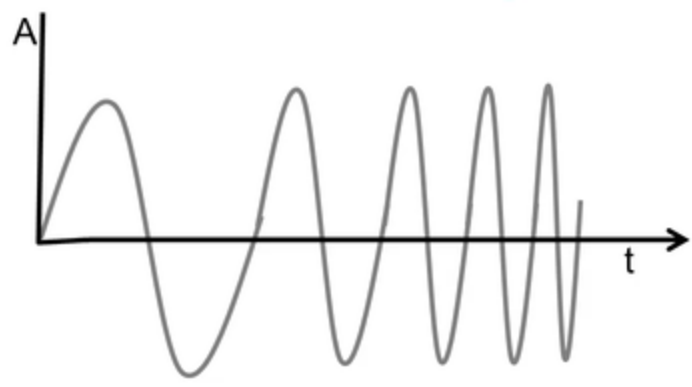
\includegraphics[ width=0.7\linewidth, keepaspectratio]{chirp_a_vs_t.png}
			\caption{Linearly modulated sinusoidal signal known as a chirp. Modulates from frequency $f_c$ to $f_c + B$ \cite{tiPresentation}.}
			\label{fig:chirp_a_vs_t}
		\end{figure} %

		Originally, the sensor itself was designed as a camera which would use computer vision algorithms to identify the region of the grooves in the tread, using either a laser or a stereo camera setup to determine depth in the received image. This would allow for good accuracy in the depth measurement. However, we quickly identified issues with this design. Most importantly, adverse environmental conditions seen under wheel wells would make it extremely difficult for the camera to see the grooves in the tread. Dirt, mud, and water kicked up by the wheel would require the camera to be regularly cleaned by the driver. Frequent upkeep is generally not viewed positively by consumers. For these reasons, an optical camera based sensor was scrapped.

		The current design of the sensor uses radar sensing techniques. With radar, dirt, mud, water, and low-light conditions do not affect the sensor's accuracy. The system can also measure much more accurately and consistently. However, this does come at an increased price over the optical sensors. 

		To measure the tread depth, a radar sensor is used. There are many different types of radar sensing that have different characteristics and different distance sensing methods. Pulsed Coherent Radar is a very simple type of radar sensing that sends out pulsed signals, meaning that the transmitter briefly emits a pulse and the receiver then listens to determine how long it takes for the pulse to respond. One of the most popular off-the-shelf parts utilizing this radar technology is the Acconeer A111 chip \cite{A111}. Unfortunately, this chip contains only one receiver. This allows only for simple object detection (e.g., waving a hand or moving an object). For a radar system to properly map a surface, there must be multiple receivers on the device. Because of this, and our lack of equipment to fully design and create a millimeter-wave radar system, we must instead move to Frequency Modulated Continuous Wave (FMCW) radar \cite{roleOfmmWave,high-accuracy,understanding,thesis,experiment}.

		\begin{figure}[t]
			\centering
			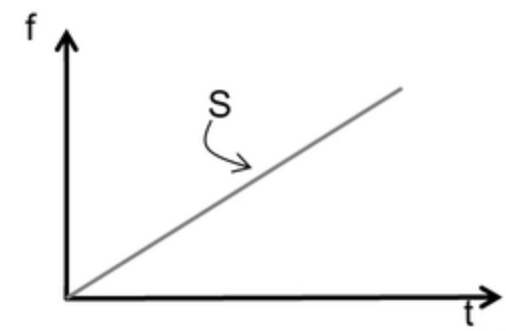
\includegraphics[ width=0.7\linewidth, keepaspectratio]{chirp_f_vs_t.png}
			\caption{Chirp in a frequency vs time plot showing the linear modulation with slope $S$ \cite{tiPresentation}.}
			\label{fig:chirp_f_vs_t}
		\end{figure} %

		\begin{figure}[t]
			\centering
			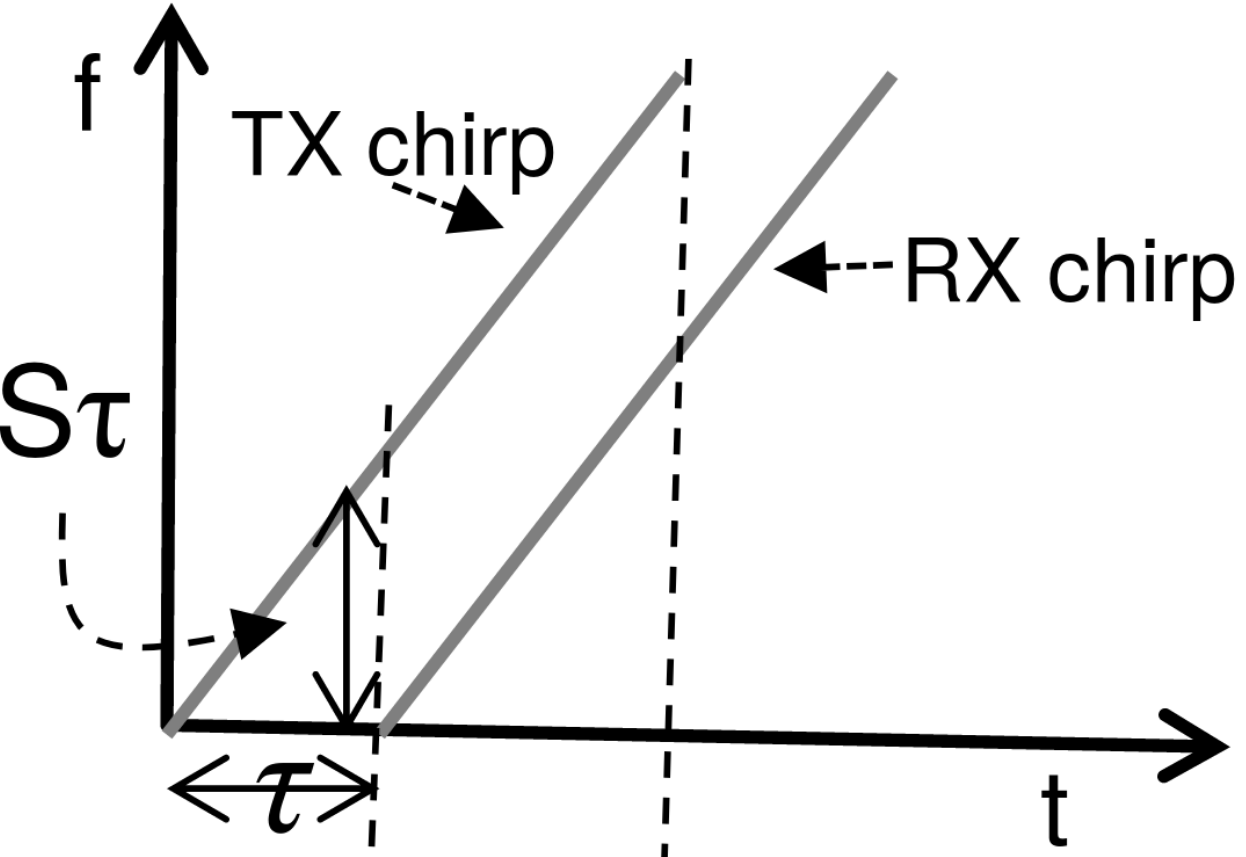
\includegraphics[ width=0.7\linewidth, keepaspectratio]{tx_rx_chirp.png}
			\caption{Showcasing time difference $\tau$ between transmitted and received chirp \cite{tiPresentation}.}
			\label{fig:tx_rx_chirp}
		\end{figure} %

		FMCW radars generate a sinusoidal signal whose frequency is linearly modulated over bandwidth $B$ from the center frequency $f_c$ to $f_c + B$ as shown in \autoref{fig:chirp_a_vs_t}. This signal is known as a chirp. The rate of increase $S$ in the frequency, also known as sweep rate, is given in MHz/s. The time span over which the signal is modulated is given by $T_c$ in seconds. \autoref{fig:chirp_f_vs_t} shows the frequency of the chirp over time.

		The receiver modules then receive the chirp after it has traveled to an object and bounced back. The time difference between when the chirp is first transmitted and when it is first received is given by $\tau$ as shown in \autoref{fig:tx_rx_chirp}. The signal being transmitted at time $t$ has the frequency $\omega_1$ while the signal being received at the same time has frequency $\omega_2$. By sending the currently transmitted and received chirps through a mixer, an Intermediate Frequency (IF) signal is produced. The instantaneous frequency of the IF signal is the difference of the instantaneous frequencies of the two chirps. The frequency of the IF signal $S_{\tau}$ is then $\frac{S2d}{c}$. This value is a constant as the difference between the transmitted and received chirps will always be the same. The IF signal can be determined using the transmit chirp $x_{TX}$ and the receive chirp $x_{RX}$ to create $x_{IF}$ as follows:
		\begin{align}
			x_1 	&= \text{sin}[\omega_1t + \phi_1] \label{eq:x1} \\
			x_2 	&= \text{sin}[\omega_2t + \phi_2] \label{eq:x2} \\
			x_{out} &= \text{sin}[(\omega_1 - \omega_2)t + (\phi_1 - \phi_2)]. \label{eq:xout}
		\end{align}

		Using the frequency of the IF signal $f_{IF}$, the distance of an object $d$ can be calculated using the equation
		\begin{equation}
			d = \frac{cf_{IF}}{2S}.
		\end{equation}

		Since the received chirp will bounce off both the surface of the tread and the grooves from different angles, the resulting received chirp will have multiple frequency components. Each of these components will correspond to different points on the tire. It is important to differentiate these points to form an accurate mapping of the surface of the tire. 

		\begin{figure}[tbp]
			\centering
			\begin{subfigure}[b]{\linewidth}
				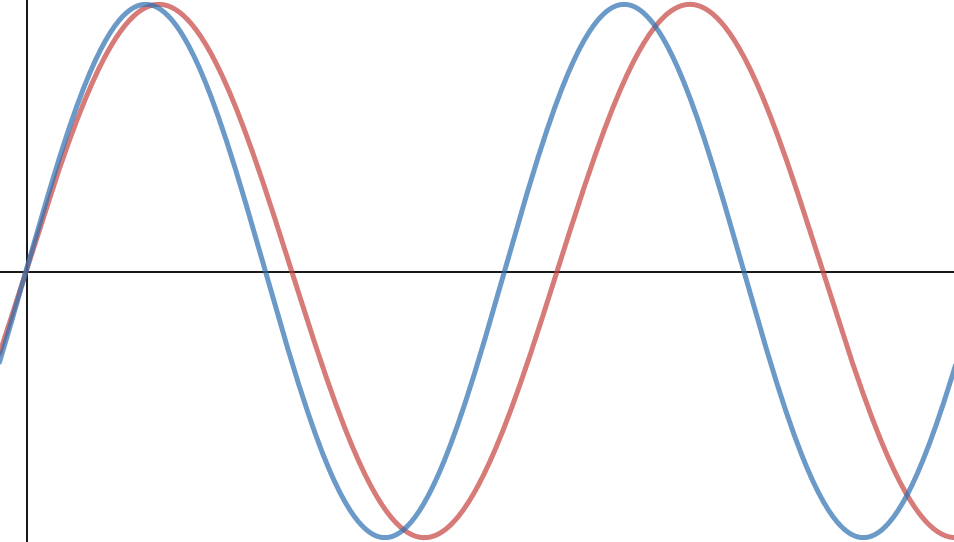
\includegraphics[width=0.5\linewidth,keepaspectratio]{shortSine.png}
				\caption{}
				\label{fig:shortSine}
			\end{subfigure} %
			\begin{subfigure}[b]{\linewidth}
				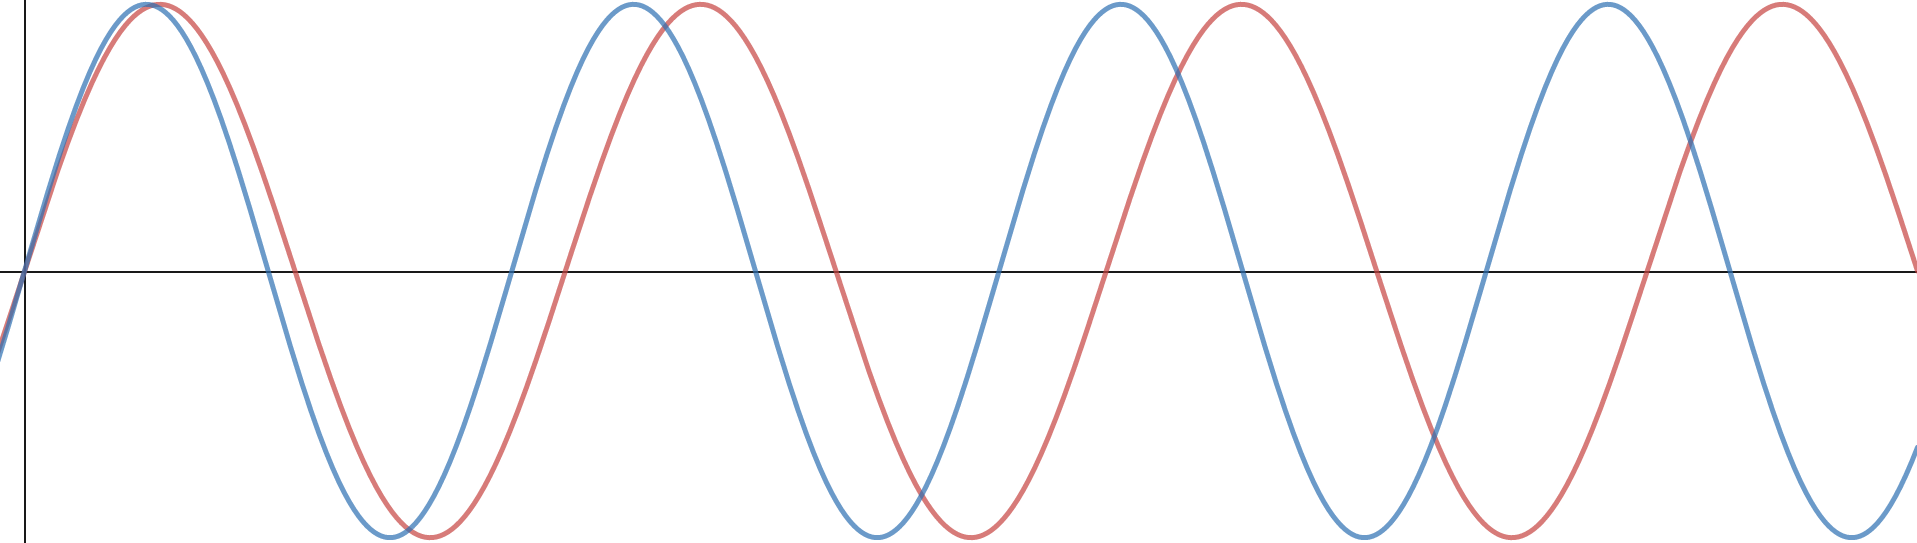
\includegraphics[width=\linewidth,keepaspectratio]{longSine.png}
				\caption{}
				\label{fig:longSine}
			\end{subfigure} %
			\caption{Observing a fewer number of cycles (a) versus observing more cycles (b) does not give enough resolution to determine the difference between two objects.}
			\label{fig:LongvShortSine}
		\end{figure}%

		By performing a fourier transform of the chirp, the different frequency components will be determined. However, because of the very small difference in distance between the surface of the tread and the grooves, these frequencies will be very close together. To be able to differentiate between these frequencies, a long observation window is required. By increasing the observation window time, the range resolution increases. This can be seen by comparing the plots of two sine waves with similar, but different frequencies over a short period of time, \autoref{fig:shortSine}, and over a longer period of time, \autoref{fig:longSine}. From these figures, it is obvious that a longer observation window shows the sine waves are significantly different, implying multiple objects at different distances.

		Using all of this information provides us with a distance to an object. However, this does not provide us with a direction to the object. That is, finding the frequencies of the received chirps will tell us how far away objects are, but not whether they are to the right or to the left of us. To do this, we need to estimate the Angle of Attack (AoA) of the received signals. This is done by comparing the signals received at at least two different receivers. This is the same concept as stereo vision where having two or more perspectives allows for depth perception by comparing the information the two receivers receive. 

		\begin{figure}[tbp]
			\centering
			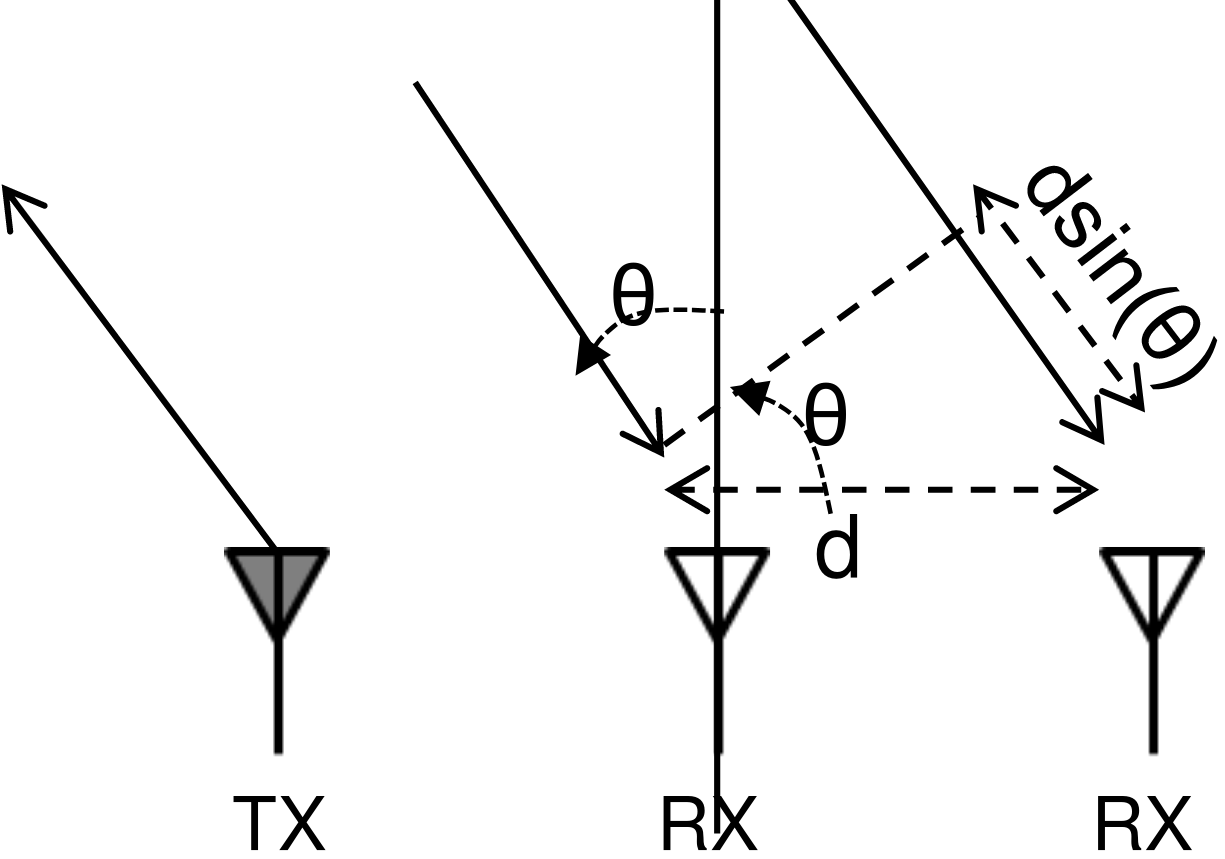
\includegraphics[ width=0.7\linewidth, keepaspectratio]{aoaFig.png}
			\caption{Angle of attack showcase using one transmitter and two receivers \cite{tiPresentation}.}
			\label{fig:aoa}
		\end{figure} %

		Each of the receivers perform a 2-dimensional FFT on the received data to produce a grid result where signals are binned based on range and velocity. For each receiver, signals in the same location will have frequency peaks at the same point. However, they will have different phases due to their incoming AoA for each receiver. The phase difference between these two signals is given by $\omega$. Then, the AoA, given by $\theta$, can be calculated using $\omega = \frac{2\pi\text{sin}(\theta)}{\lambda}$. This can be derived from \autoref{fig:aoa} which shows two receiver modules receiving a chirp bounced from the same object. 

		\begin{figure}[tbp]
			\centering
			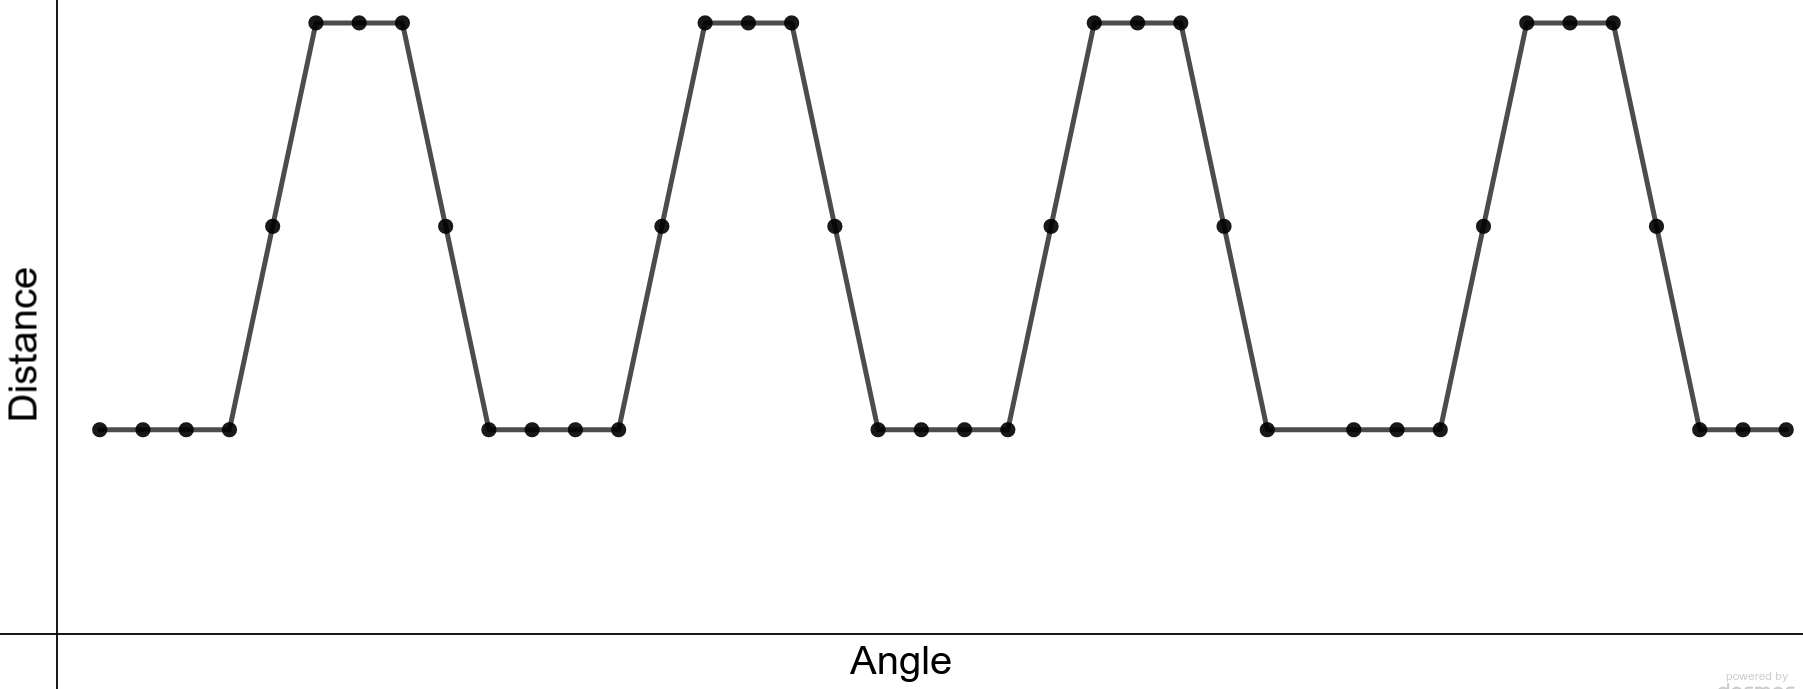
\includegraphics[ width=\linewidth, keepaspectratio]{treadMap.png}
			\caption{Example tread mapping where the y-axis is the distance from the sensor and the x-axis is the angle to the sensor. The peaks are the grooves in the tire (further away) while the points in the troughs represent the surface of the tread (close to the sensor).}
			\label{fig:treadMap}
		\end{figure} %

		Combining the AoA information with the range detection, data points can be collected horizontally across the tire as other data is filtered out. This data can be plotted to form a mapping of the surface of the tread on the tire. An example of this is shown in \autoref{fig:treadMap}. This plot shows the distance at points on the tread of the tire where points further away represent the grooves and points closer to the sensor represent the surface of the tread. The x-axis represents the angle of attack from the measured point to the sensor. 

		The system will then take an average of the high points and the low points and find the difference between the two. This gives an average tread depth reading. If this value is outside of the acceptable range (usually less than 3/32'' on passenger vehicles), then the user will be notified that the tread depth is dangerously low. This notification will likely take the form of an LED within the car itself. Further integration into the dashboard is possible, but requires significant customization of the vehicle until car manufacturers adopt tread awareness systems as standard.


	\section{Parts List}
		Our design consists of two main parts: an FMCW radar sensor and a microcontroller for debugging and rapid prototyping. Additionally, for the prototype stage, we will use a simple LED output to display whether the tire tread depth is outside of a predetermined safe range. For the FMCW radar sensor, we have selected Texas Instruments' AWR1843BOOST FMCW radar sensor evaluation module. This module consists of the AWR1843 FMCW radar sensor processor with integrated ARM Cortex-R4F microcontroller, C674X DSP, 2 MB of on-chip memory, as well as multiple communication interfaces including SPI and CAN-FD to allow communication to microcontrollers and to a vehicle's central communication system.

		For the microcontroller, we have selected an MSP432 LaunchPad. This is mainly due to the fact that the AWR1843BOOST is designed specifically to interface well with the LaunchPad ecosystem of microcontrollers for ease of use. Other microcontrollers, such as Raspberry Pis, are available to use. However, TI also provides a simple mmWave SDK as well as a customized development environment based off of the Eclipse IDE to facilitate the design process. 

		\autoref{tab:parts} lists the parts choices we have made for this design including their price and quantity. The AWR1843BOOST package includes mounting brackets, rubber bump-ons for stabilization, and a USB cable to interface with the microcontroller or a computer. The team already has multiple MSP432s and so does not need to purchase additional items. However, the price is included in the table to accurately represent the full cost of the prototype system. The shipping price when ordering both the AWR1843BOOST and MSP432 directly from TI online is at minimum \$6.99. This brings the total cost of the product, pre-tax, to \$325.98. Following, we discuss the process of selecting the AWR1843 FMCW radar sensor. 

		\begin{table}[t]
			\begin{center}
				\caption{Parts required for ATIS using a radar sensor.}
				\label{tab:parts}
				\begin{tabular}{l|l|l}
					Part/Expense		& Quantity 	& Cost  	\\
					\hline
					\vspace{-0.1in}		&			&			\\
					AWR1843BOOST 		& 1 		& \$299.00	\\
					MSP-EXP432P401R		& 1 		& \$19.99	\\
					Red LED 			& 1 		& \$0.35	\\
					Shipping 			& -			& \$6.99 	\\
					\hline
					\vspace{-0.1in}		&			&			\\
					\textbf{Total} 		& 3			& \$325.98
				\end{tabular}
			\end{center}
		\end{table}

		\subsection{FMCW Radar Sensor}
			\label{ssec:FMCW}
			To determine which FMCW radar sensor would best suit the design, requirements, and specifications of ATIS, we first researched what companies offer FMCW radar solutions. There are many companies that offer FMCW products (e.g., \cite{fluidic,liteye,houston,analog,nxp}). However, most of these products are either too specific in purpose \cite{liteye}, not accurate enough \cite{houston}, in a lower frequency band than required \cite{analog}, or is not included in an evaluation board \cite{nxp}. 

			\begin{table*}[t]
				\begin{center}
					\caption{Device comparison for AWR1xxx mmWave processors.}
					\label{tab:processors}
					\begin{tabular}{l|l|l|l|l|l}
						Functionality 								& AWR1243 		& AWR1243P 		& AWR1443 		& AWR1642 		& AWR1843 	\\
						\hline
						\vspace{-0.1in}								&				&				&				&				&			\\
						Number of Receivers 						& 4				& 4				& 4				& 4				& 4			\\
						Number of Transmitters						& 3				& 3				& 3				& 2				& 3			\\
						Simultaneous Transmitters					& 2				& 3				& 2				& 2				& 3			\\
						On-Chip Memory 								& -				& -				& 576 KB 		& 1.5 MB 		& 2 MB 		\\
						Max real sampling rate (Msps)				& 37.5 			& 37.5			& 12.5			& 12.5			& 25		\\
						Max complex sampling rate (Msps)			& 18.75			& 18.75			& 6.25			& 6.25			& 12.25		\\
						Micro Controller Unit (R4F)					& -				& -				& Yes 			& Yes 			& Yes 		\\
						Digital Signal Processor (C674X)			& -				& -				& - 			& Yes 			& Yes 		\\
						Serial Peripheral Interface (SPI) Ports 	& 1				& 1				& 1				& 2				& 2			\\
						Quad Serial Peripheral Interface (QSPI) 	& -				& -				& Yes 			& Yes 			& Yes 		\\
						Inter-Integrated Circuit (I$^\text{2}$C) 	& -				& -				& Yes 			& Yes 			& Yes 		\\
						Controller Area Network (DCAN) interface 	& -				& -				& Yes 			& Yes 			& Yes 		\\
						CAN FD 										& - 			& -				& - 			& Yes 			& Yes 		\\
						JTAG 										& - 			& - 			& Yes 			& Yes 			& Yes 		\\
					\end{tabular}
				\end{center}
			\end{table*}

			For automotive applications in the 77GHz band, Texas Instruments (TI) and NXP are the leaders in FMCW radar chips. NXP produces one FMCW chip \cite{nxp}, however it is only sold as a BGA chip which is outside of our skill set to use. This led us to choose TI as our product source. TI produces a large product line of FMCW chips which are also made available in evaluation modules, also called booster packs. 

			These modules are developed specifically to integrate with the TI LaunchPad ecosystem. These evaluation boards have SPI, I2C, and UART capabilities, enabling communication with other microcontrollers such as a Raspberry Pi. TI also supplies a mmWave SDK \cite{sdk} that integrates with their development environment Code Composer Studio, a custom version of the Eclipse IDE. This allows developers to rapidly prototype system programs for their mmWave devices.

			TI offers a large selection of evaluation modules (EVM) for their FMCW device families. These EVMs are designed with direct connectivity to TI's MCU LaunchPad ecosystem for simple, rapid prototyping. The EVM boards include onboard emulation for programming and debugging, onboard buttons, and LEDs for quick integration of a simple user interface.

			The TI booster packs are broken into two device families. The AWR family covers automotive applications \cite{awr} while the IWR family covers industrial applications. Based on their functionality, the two families are the same. Although most of the AWR applications can be performed on the IWR booster packs, the AWR booster packs are more qualified for automotive applications as they are AEC-Q100-qualified and nealy all are Automotive Safety Integrity Level B-type (ASIL-B) targeted. This is not the case for the IWR devices as these qualifications are not required for industrial applications. AEC-Q100 is a failure mechanism-based stress test qualification for integrated circuits used in automotive applications and guarantees a certain level of quality and reliability \cite{aecq100}. ASIL is a risk classification system defined by the ISO 26262 standard \cite{iso26262} for the safety of vehicles and ranges from ASIL-A to ASIL-D. Products with ASIL-A classification pose the least amount of risk while ASIL-D classified products pose the highest potential for life-threatening or fatal injury in the event of a malfunction in the device \cite{asil}. 

			Both device families have a lower bound operating temperature of \ang{-40}C. The AWR family has a higher upper bound of +\ang{125}C to prevent damage while exposed to the environment with little to no protection compared to the IWR family's +\ang{105}C upper limit. 

			Given these key differences between the AWR and IWR device families, we have chosen the AWR family for our application. This is mainly due to the higher safet and quality standards, as the two families do not differ in other functional aspects. The AWR device family consists of the AWR1243, AWR1243P, AWR1443, AWR1642, and AWR1843. Each of these processors contain mmWave radar sensors that function in the 76 to 81 GHz band with a 4 GHz available bandwidth. They are each also sold in EVMs to allow for easier prototyping. Since each of the EVM packages add the same functionality, we only considered differences in the processors themselves to make a final decision. \autoref{tab:processors} summarizes the key specifications of each of the processors and detailed breakdowns of each processor follow.

			\subsubsection{AWR1243/AWR1243P}
				The only difference between the AWR1243 and AWR1243P devices \cite{awr1243,awr1243boost} is that the AWR1243P supports a three TX simultaneous operation while the AWR1243 only supports a two TX simulatenous operation. Based ont he specifications and requirements, the three TX simultaneous operation is not necessary as we will only need to transmit two signals at a given time. The advantage of these two processors is that both have a maximum real sampling rate of 37.5 Msps and a maximum complex sampling rate of 18.75 Msps. This measurement is the number of samples taken per second and is important for recording an accurate waveform of the received signal.

				The first major disadvantage is that both processors do not have an internal processor-based MCU nor a digital signal processor (DSP). A basic MCU incorporates teh CPU, memory, and peripheral functions while a DSP is used to measure, filter, or compress continuous analog signals. The second major disadvantage is that neither have on-chip memory which is crucial in decreasing latency for critical and frequently used data. With this in mind, on-chip memory can oftsen save development time and cost \cite{memory}.

				The third major disadvantage is that although both booster packs have a serial peripheral interface (SPI) port, neither supports the Joint Test Action Group (JTAG) protocol. The JTAG protocol primarily functions by enabling communication with an MCU during product development, emulation, and application debugging \cite{jtag}.

				The fourth major disadvantage is that both processors do not have a quad serial peripheral interface (QSPI). This would provide the necessary support for communicating with an external flash memory device using SPI, which would greatly assist in retaining data for comparison to ensure that readings are accurate. The last major disadvantage is that neither supports the controller area network (CAN) protocol nor the controller area network with flexible data rate (CAN-FD) protocol. The CAN protocol provides an inexpensive and durable network to allow multiple CAN devices to communicate with one another \cite{iso11898}. CAN-FD improves on the standard CAN protocol by allowing up to 64-bytes in a single message, greatly improving the data throughput. 

				The AWR1243 and AWR1243P have the best in class sampling rates. However, they are missing multiple crucial communication protocols QSPI, I$^\text{2}$C, CAN, and CAN-FD which prevents the device from effectively communicating with a vehicle. Additionally, these devices do not have an on-board MCU or DSP, making prototyping more difficult as they can not be directly programmed.

			\subsubsection{AWR1443}
				Similar to the AWR1243 and AWR1243P, the AWR1443 \cite{awr1443,awr1443boost} has four RX channels and three TX channels. However, it only supports operation of two simultaneous TX channels. A major disadavantage for this processor is that there is not an on-board DSP.  However, it does have an ARM Cortex-R4F MCU. This processor has a lower real and complex sampling rate than the AWR1243, potentially leading to less accurate results. The main advantages of the AWR1443 is 576 KB of on-chip memory and support of the JTAG, DCAN, I$^\text{2}$C, SPI, and QSPI communication protocols. Because of the additional communication capabilities of this processor as well as the on-board MCU, it is considered over the AWR1243 and AWR1243P for this design.

			\subsubsection{AWR1642}
				The AWR1642 \cite{awr1642,awr1642boost} has four RX channels, similar to the previously considered processors. However, the AWR1642 only has two TX channels. Compared to the AWR1443, this processor has the same maximum real and complex processing rates of 12.5 and 6.25 Msps, respectively. The major advantages the AWR1642 has over the AWR1443 is that it has a larger on-chip memory of 1.5 MB and supposerts the higher throughput CAN-FD protocol. Because of these small advantages, we can rule out the AWR1443 and instead consider the AWR1642 for our design.

			\subsubsection{AWR1843}
				The AWR1843 \cite{awr1843,awr1843boost} is one of TIs most recent mmWave developments, having been released in Fall of 2019. This processor has four RX and three TX channels and also supports all three TX channels in simultaneous operation. The AWR1843 contains an integrated ARM Cortex-R4F MCU and C674X DSP unit. Similar to the AWR1642, this processor supports JTAG, SPI, QSPI, DCAN, and CAN-FD protocol interfaces. It's main advantage over the AWR1642 is that its max real and complex sampling rates are doubled at 25 and 12.25 Msps, respectively. Additionally, it has a larger on-board chip memory of 2 MB compared to the AWR1642s 1.5 MB. Based on these findings, we can select the AWR1843 as the processor to use for our FMCW radar design as it best suits the design, requirements, and specifications of ATIS. 


	\section{Prototype and System Integration}
		By the end of this semester, our expectation is to have a working prototype of an FMCW radar sensor to map the surface of a tire. The sensor will send the data to a microcontroller that will then determine the approximate tread depth. The controller will then send a notification signal (likely through an LED for prototyping) to alert a driver if the tread depth is outside of a specified range.

		Once these functionalities are implemented, the sensor will be improved to measure with a higher accuracy. Then, functional tests on a real vehicle will be conducted. From this point, optimization and further testing will be conducted to improve the device. The housing of the sensor will also be improved so that inclement weather, rough terrain, and dirt do not degrade the measurements taken. Through this process, the sensor will be made with off-the-shelf parts to stay within budget and produce a working final product.


	\section{Deliverables}
		By the end of the project timeline, the final product will be able to accurately detect tread depth on a passenger vehicle tire to an accuracy less than or equal to 2/32''. The device will be mountable on a vehicle's wheel well. A potential implementation would be to integrate the device with a vehicle's CAN communication system to allow the device to communicate with the vehicle to send upadtes to the operator.

		Once the product itself is complete, we will compose a final report discussing our findings, results, and conclusions. This report will discuss the specifics of the final product, the difficulties in completing it, and the specific details of how it functions. A poster and presentation will also be prepared to give a high-level understanding of the product and how it functions to business leaders, professors, and peers.


	\section{Timeline}
		To ensure the timely completion of the project, three Gantt charts have been created. These charts supply us with expected milestones for the project. This allows us to visually determine whether or not we are on schedule to complete the project. The Gantt chart is a constantly adjusting figure that will become more specific as the design for the product is further refined. \autoref{fig:ganttChartSP2020}, \autoref{fig:ganttChartSU2020}, and \autoref{fig:ganttChartFA2020} are the Gantt charts outlining our planned tasks over the spring, summer, and fall of 2020, respectively.

		\begin{figure*}[t]
			\centering
			\begin{ganttchart}[y unit title=0.5cm, y unit chart=0.6cm, x unit=0.75cm, vgrid, hgrid, title label anchor/.style={below=-1.6ex}, title left shift=0, title right shift=0, title height=1, bar/.style={fill=gray!50}, incomplete/.style={fill=white}, progress label text={}, bar height=0.5, group right shift=0, group top shift=.6, group height=.3]{1}{17}
				% Month labels
				\gantttitle{January}{3}
				\gantttitle{February}{4} 
				\gantttitle{March}{5} 
				\gantttitle{April}{4} 
				\gantttitle{May}{1}  \\

				% First day of week labels
				\gantttitle{13}{1}
				\gantttitle{20}{1}
				\gantttitle{27}{1}

				\gantttitle{3}{1}
				\gantttitle{10}{1}
				\gantttitle{17}{1}
				\gantttitle{24}{1}

				\gantttitle{2}{1}
				\gantttitle{9}{1}
				\gantttitle{16}{1}
				\gantttitle{23}{1}
				\gantttitle{30}{1}

				\gantttitle{6}{1}
				\gantttitle{13}{1}
				\gantttitle{20}{1}
				\gantttitle{27}{1}

				\gantttitle{4}{1} \\

				% Tasks
				% To set color use [bar/.append style = { fill = $(COLOR) } ]
				\ganttbar{Project Proposal}{1}{16} 		\\ % January 13 - April 27
				\ganttbar{Sensor Design}{4}{17} 		\\ % February 3 - May 4
				\ganttbar{Order Parts}{15}{17} 			\\ % April 20 - May 4
				\ganttbar{Initial Construction}{16}{17}    % April 27 - May 4

				% Relations 
				% \ganttlink{elem1}{elem4}
				% \ganttlink{elem2}{elem4}
				% \ganttlink{elem3}{elem4}
			\end{ganttchart}
			\caption{Tasks for Spring 2020.}
			\label{fig:ganttChartSP2020}
		\end{figure*}

		\begin{figure*}[t]
			\centering
			\begin{ganttchart}[y unit title=0.5cm, y unit chart=0.6cm, x unit=0.85cm, vgrid, hgrid, title label anchor/.style={below=-1.6ex}, title left shift=0, title right shift=0, title height=1, bar/.style={fill=gray!50}, incomplete/.style={fill=white}, progress label text={}, bar height=0.5, group right shift=0, group top shift=.6, group height=.3]{1}{15}
				% Month labels
				\gantttitle{May}{3}
				\gantttitle{June}{5} 
				\gantttitle{July}{4} 
				\gantttitle{August}{3} \\

				% First day of week labels
				\gantttitle{11}{1}
				\gantttitle{18}{1}
				\gantttitle{25}{1}

				\gantttitle{1}{1}
				\gantttitle{8}{1}
				\gantttitle{15}{1}
				\gantttitle{22}{1}
				\gantttitle{29}{1}

				\gantttitle{6}{1}
				\gantttitle{13}{1}
				\gantttitle{20}{1}
				\gantttitle{27}{1}

				\gantttitle{3}{1}
				\gantttitle{10}{1}
				\gantttitle{17}{1} \\

				% Tasks
				\ganttbar{Initial Construction}{1}{3} \\ % 
				\ganttbar{Housing Design}{7}{10} 		\\ % 
				\ganttbar{Alert System Design}{8}{12} 	\\ % 
				\ganttbar{Redesign}{4}{8} \\
				\ganttbar{Initial Testing}{2}{4} \\
				\ganttbar{Redesign Testing}{7}{9} \\
				\ganttbar{\quad\quad\enspace Final Redesign}{8}{15}

				% Relations 
				% \ganttlink{elem0}{elem1}
			\end{ganttchart}
			\caption{Tasks for Summer 2020.}
			\label{fig:ganttChartSU2020}
		\end{figure*}

		\begin{figure*}[t]
			\centering
			\begin{ganttchart}[y unit title=0.5cm, y unit chart=0.6cm, x unit=0.796875cm, vgrid, hgrid, title label anchor/.style={below=-1.6ex}, title left shift=0, title right shift=0, title height=1, bar/.style={fill=gray!50}, incomplete/.style={fill=white}, progress label text={}, bar height=0.5, group right shift=0, group top shift=.6, group height=.3]{1}{16}
				% Month labels
				\gantttitle{August}{2}
				\gantttitle{September}{4} 
				\gantttitle{October}{4} 
				\gantttitle{November}{5} 
				\gantttitle{Dec.}{1}  \\

				% First day of week labels
				\gantttitle{24}{1}
				\gantttitle{31}{1}

				\gantttitle{7}{1}
				\gantttitle{14}{1}
				\gantttitle{21}{1}
				\gantttitle{28}{1}

				\gantttitle{5}{1}
				\gantttitle{12}{1}
				\gantttitle{19}{1}
				\gantttitle{26}{1}

				\gantttitle{2}{1}
				\gantttitle{9}{1}
				\gantttitle{16}{1}
				\gantttitle{23}{1}
				\gantttitle{30}{1}

				\gantttitle{7}{1} \\

				% Tasks
				\ganttbar{Final Redesign}{1}{2} \\
				\ganttbar{Product Testing}{1}{14} \\
				\ganttbar{Implementation}{3}{14} \\
				\ganttbar{Optimization}{4}{12} \\
				\ganttbar{\quad Final Presentation}{12}{16}

				% Relations 
				% \ganttlink{elem0}{elem1}
			\end{ganttchart}
			\caption{Tasks for Fall 2020.}
			\label{fig:ganttChartFA2020}
		\end{figure*}

		\subsection{Teamwork}
			The timeline of the project can be broken into various phases. Although each team member will provide an equal amount of contribution, each will take a lead on a different phase of the project. The key project phases along with leaders of each phase is shown in \autoref{tab:phaseLeaders}. The ultimate goal is to be completed with the design of our prototype after the first semester. This will allow for testing and further optimization of the product during the implementation phase. This timeline will also allow extra time for unexpected issues that will arise during implementation.

			\begin{table}[tb]
				\centering
				\caption{Leaders for each key project phase.}
				\label{tab:phaseLeaders}
				\begin{tabularx}{\linewidth}{l|l}
					Project Phase 						& Leader \\
					\hline
					\vspace{-0.1in}						& \\
					Research 							& Nicholas Chiapputo \\
					Project Definition					& Brandon Jones \\
					Specification and Requirements 		& Tim McCoig \\
					Design and Algorithm Development 	& Nicholas Chiapputo \\
					Testing and Optimization 			& Brandon Jones \\
					Prototype Implementation 			& Samuel Simmons
				\end{tabularx}
			\end{table}


	\begin{thebibliography}{00}
		% Introduction
			\bibitem{cdcKeyStats} Center for Disease Control and Prevention, ``Key Data and Statistics,'' 2015. [Online]. Available: \url{https://www.cdc.gov/injury/wisqars/overview/key_data.html}

			\bibitem{nhtsaCrashStats} National Highway Traffic Safety Administration, ``Tire-Related Factors in the Pre-Crash Phase,'' 2012. [Online]. Available: \url{https://crashstats.nhtsa.dot.gov/Api/Public/ViewPublication/811617}


		% Current Products
			% \bibitem{justwheelsPatent} T. Scheckter, ``Radar tread sensing for wheel well,'' U.S. Patent 20200031173A1, Jul., 19, 2019. 
		
			\bibitem{continentalPatent} T. A. Brey, ``Tire tread wear sensor system,'' U.S. Patent 7180409B2, Feb., 20, 2007.
			
			\bibitem{intellitread} ``Tire Tread Wear Sensors - Tyrata.'' Accessed on: Feb. 11, 2020. [Online]. Available: \url{https://tyrata.com/}
			
			\bibitem{goodyearPatent1} C. T. R. Pulford, C. H. Lin, ``Sensor system for monitoring tire wear,'' U.S. Patent 20190184763A1, Dec., 19, 2018.
			
			\bibitem{nxpbvPatent} R. L. Robinson, ``System and method for determining tread wear of a tire,'' U.S. Patent 9831922B1, Nov., 28, 2017.
			
			\bibitem{goodyearPatent2} M. Engel, B. W. Kimble, and D. Lednik, ``Tire tread wear sensor system,'' U.S. Patent 20160075189A1, Mar., 17, 2014.
			
			\bibitem{patent4} R, Achterholt, ``Method and device for detecting the wear on at least one tire of a vehicle,'' U.S Patent 20190344625A1, Nov., 14, 2019.


		% Constraints
			% SiGe papers
				\bibitem{122ghz} S. Scherr, \textit{et al.}, ``Miniaturized 122 ghz ism band fmcw radar with micrometer accuracy,'' In \textit{2015 European Radar Conference (EuRAD)}, Paris, 2015, pp. 277-280.

				\bibitem{240ghz} T. Jaeschke, C. Bredendiek, N. Pohl. ``A 240 ghz ultra-wideband fmcw radar system with on-chip antennas for high resolution radar imaging,'' In \textit{2013 IEEE MTT-S International Microwave Symposium Digest (MTT)}, Seattle, WA, 2013, pp. 1-4.
    	

		% Standards
			\bibitem{etsi-reduced-24ghz} ``ETSI EN 302 288 - ultra-wideband radar equipment operating in the 24,25 GHz to 26,65 GHz range,'' European Telecommunications Standards Institute, May 2015. [Online].Available: \url{https://www.etsi.org/deliver/etsi_en/302200_302299/302288/02.01.01_60/en_302288v020101p.pdf} (accessed Apr. 22, 2020).

			\bibitem{fcc-15-16} ``FCC 15-16,'' Federal Communications Commission FCC 15-16, Feb. 2015. [Online].Available: \url{https://apps.fcc.gov/edocs_public/attachmatch/FCC-15-16A1_Rcd.pdf} (accessed Apr. 22, 2020).

			\bibitem{fcc-76-81} ``Radar services in the 76-81 ghz band,'' Federal Communications Commission, Jun. 2017. [Online].Available: \url{https://www.fcc.gov/document/radar-services-76-81-ghz-band} (accessed Apr. 22, 2020).

			\bibitem{etsi-76-77} ``ETSI EN 301 091-2 - Radar equipment operating in the 76 ghz to 77 ghz range,'' European Telecommunications Standards Institute, Jan. 2017. [Online].Available: \url{https://www.etsi.org/deliver/etsi_en/301000_301099/30109102/02.01.01_60/en_30109102v020101p.pdf} (accessed Apr. 22, 2020).

			\bibitem{etsi-77-81} ``ETSI EN 302 264-1 - Short range radar equipment operating in the 77 ghz to 81 ghz band,'' European Telecommunications Standards Institute, Jun. 2009. [Online].Available: \url{https://www.etsi.org/deliver/etsi_en/302200_302299/30226401/01.01.01_60/en_30226401v010101p.pdf} (accessed Apr. 22, 2020).

			\bibitem{ti-24-77} ``Moving from legacy 24 ghz to state-of-the-art 77 ghz radar,'' Texas Instruments, Oct. 2017. [Online].Available: \url{https://www.ti.com/lit/wp/spry312/spry312.pdf} (accessed Apr. 22, 2020).

			\bibitem{iso26262} \textit{Road Vehicles - Functional Safety}, ISO 26262-1:2018, International Organization for Standardization, Dec. 2018.

			\bibitem{asil} ``What is the ISO26262 functional safety standard?,'' ni.com. [Online].Available: \url{https://www.ni.com/en-us/innovations/white-papers/11/what-is-the-iso-26262-functional-safety-standard-.html#toc2} (accessed Apr. 22, 2020).

	    	\bibitem{aecq100} \textit{Failure Mechanism Based Stress Test Qualification for Integrated Circuits}, AECQ100, Automotive Electronics Council, Sept. 2014. [Online].Available: \url{http://aecouncil.com/Documents/AEC_Q100_Rev_H_Base_Document.pdf}.


		% Design
			% Products
				\bibitem{A111} ``SparkFun Pulsed Radar Breakout - A111.'' SparkFun. \url{https://www.sparkfun.com/products/15577} (accessed Mar. 9, 2020).

			% Academic/Scholarly Papers
				\bibitem{roleOfmmWave} A. Bhutani, S. Marahrens, M. Gehringer, B. G{\"o}ttel, M. Pauli, and T. Zwick, ``The role of millimeter-waves in the distance measurement accuracy of an fmcw radar sensor,'' \textit{Sensors 2019}, vol. 19, no. 18, Sept., 2019, doi: 10.3390/s19183938.

				\bibitem{high-accuracy} P. Pahl, T. Kayser, M. Pauli, and T. Zwick, ``Evaluation of a high accuracy range detection algorithm for FMCW/phase radar systems,'' In \textit{The 7th European Radar Conference}, Paris, 2010, pp. 160-163.

				\bibitem{understanding} G. M. Brooker, ``Understanding millimetre wave FMCW radars,'' In \textit{1st International Conference on Sensing Technology}, Palmerston North, New Zealand, 2005, pp. 152-157.

				\bibitem{thesis} J. L. Uphoff, ``Introduction to automotive FMCW radar technologies,'' M.S. thesis. Dept. of Appl. Signal Process., Blekinge Inst. of Technol., Karlskrona, Sweden, 2018.

				\bibitem{experiment} X. Gao, G. Xing, S. Roy, and H. Liu, ``Experiments with mmWave automotive radar test-bed,'' arXiv: 1912.12566 [eess.SP], Dec. 2019.
			
			% TI presentation on FMCW 
				\bibitem{tiPresentation} S. Rao. Introduction to mmwaveSensing: FMCW Radars [PDF]. Available: \url{https://training.ti.com/sites/default/files/docs/mmwaveSensing-FMCW-offlineviewing_2.pdf}.


		% Parts List
			% FMCW Companies
				\bibitem{fluidic} ``Honetwell RM60 FMCW Radar Level Transmitter.'' fluidic-ltd.co.uk. \url{https://fluidic-ltd.co.uk/product/honeywell-rm60/} (accessed Apr. 20, 2020).

				\bibitem{liteye} ``Surveillance Radar - Liteye Systems, Inc.`` liteye.com. \url{https://liteye.com/products/surveillance-radar/} (accessed Apr. 20, 2020).

				\bibitem{houston} ``PD300/PD310.'' houston-radar.com. \url{https://houston-radar.com/products/radar-data-collectors/pd300-pd310-oem-fmcw-presence-detector-radar/} (accessed Apr. 20 2020).

				\bibitem{analog} ``ADF5901.'' analog.com. \url{https://www.analog.com/en/products/ADF5901.html#product-overview} (accessed Apr. 20 2020).
				
				\bibitem{nxp} ``TEF810X Fully-Integrated 77 GHz Radar Transceiver.'' nxp.com. \url{https://www.nxp.com/products/rf/radar-transceivers/tef810x-fully-integrated-77-ghz-radar-transceiver:TEF810X} (accessed Apr. 20 2020).

			% Texas Instruments Parts Discussion
				\bibitem{sdk} mmWave software development kit (SDK). Texas Instruments. [Online].Available: \url{https://www.ti.com/tool/MMWAVE-SDK} (accessed Apr. 22, 2020)

				\bibitem{awr} Automotive mmWave Sensors. Texas Instruments. \url{https://www.ti.com/sensors/mmwave/awr/overview.html} (accessed Apr. 22, 2020).

				\bibitem{iwr} Industrial mmWave Sensors. Texas Instruments. \url{https://www.ti.com/sensors/mmwave/iwr/overview.html} (accessed Apr. 22, 2020).

				\bibitem{awr1243} AWR1243. Texas Instruments. \url{https://www.ti.com/product/AWR1243f} accessed (Apr. 22, 2020).

				\bibitem{awr1243boost} AWR1243 Single-Chip 77- and 79-GHz FMCW Transceiver. Texas Instruments. \url{https://www.ti.com/tool/AWR1243BOOST}

				\bibitem{memory} Memory System Design. Intel. \url{https://www.intel.com/content/dam/www/programmable/us/en/pdfs/literature/hb/nios2/edh_ed51008.pdf} (accessed Apr. 22, 2020).

				\bibitem{jtag} C2000 MCU JTAG Connectivity Debug. Texas Instruments. \url{https://www.ti.com/lit/spracf0}.

				\bibitem{iso11898} \textit{Road vehicles - Controller area network (CAN)}, ISO 11898-1:2015, International Organization for Standardization, Dec. 2015.

				\bibitem{awr1443} AWR1443. Texas Instruments. \url{https://www.ti.com/product/AWR1443} (accessed Apr. 22, 2020).

				\bibitem{awr1443boost} AWR1443 single-chip 76-GHz to 81-GHz automotive radar sensor evaluation module. Texas Instruments. \url{https://www.ti.com/tool/AWR1443BOOST} (accessed Apr. 22, 2020).

				\bibitem{awr1642} AWR1642. Texas Instruments. \url{https://www.ti.com/product/AWR1642} (accessed Apr. 22, 2020).

				\bibitem{awr1642boost} AWR1642 single-chip 76-GHz to 81-GHz automotive radar sensor evaluation module. Texas Instruments. \url{https://www.ti.com/tool/AWR1642BOOST} (accessed Apr. 22, 2020).

				\bibitem{awr1843} AWR1843. Texas Instruments. \url{https://www.ti.com/product/AWR1843} (accessed Apr. 22, 2020).

				\bibitem{awr1843boost} AWR1843 single-chip 76-GHz to 81-GHz automotive radar sensor evaluation module. Texas Instruments. \url{https://www.ti.com/tool/AWR1843BOOST} (accessed Apr. 22, 2020).
	\end{thebibliography}
\end{document}